% Slide 10 | Results | M4 (Vismay Shanbhag) | 0:45 | E2a: what can ADF detect?
\begin{frame}{E2a: one year sees only fast pairs}
\framesubtitle{Slide 10 \textbullet\ Results \textbullet\ M4 \textbullet\ 0:45}
\vspace{-2pt}
\begin{columns}[T,onlytextwidth]
\column{0.44\textwidth}
  \centering
  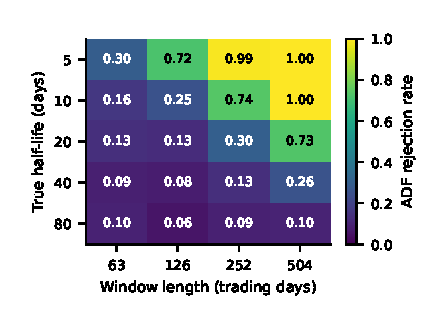
\includegraphics[width=\linewidth]{fig_e2_adf_power_report}
\column{0.52\textwidth}
  \footnotesize\raggedright
  How often ADF finds a gap that really closes, with one year of data:
  \begin{itemize}\setlength{\itemsep}{2pt}
    \item 5-day half-life: \textbf{99\%}
    \item 10 days: \textbf{74\%}
    \item 20 days: \textbf{30\%}
  \end{itemize}
\end{columns}
\pairTakeaway{Every pair we select has a half-life of 15 days or less.}
\end{frame}
